\documentclass{article}     
\usepackage[utf8x]{inputenc}
\usepackage[english,russian]{babel}
\usepackage{upgreek}
\usepackage{graphicx}
\usepackage{wrapfig}
\usepackage{amsmath}
\graphicspath{{images/}}

\begin{document}

\title{Отчет по производственной практике}
\author{Дмитриев Денис, 591 гр.}
\maketitle

Производственная практика проходила в ГАО РАН, под руковолством В.П. Гринина. Ее целью было моделирование магнитосферы молодых звезд типа Т Тельца. Магнитосфера образуется в результате падения вещества протопланетного диска на звезду, под действием сильного магнитного поля (порядка кГс). Предполагалось, что магнитное поле дипольное, что должно быть верно, если оно достаточно сильное \cite{hartmann94}. В таком случае газ будет двигаться вдоль силовых линий, форма которых определяется законом (1), где $\theta$ -- полярный угол. Скорость движения газа можно посчитать по известной формуле для падающего вещества (2)

\begin{equation}
r = r_m \sin^2 \theta
\end{equation}

\begin{equation}
v_{mz} = -v_{esc}\sqrt{\left(\frac{R_s}{r} - \frac{R_s}{r_0}\right)}
\end{equation}

Где $r_0$ -- расстояние до точки старта, а $R_s$ -- радиус звезды.
В ходе практики была успешно написана программа для расчета геометрии такой магнитосферы, используя которую можно при известных населенностях уровня расчитать профиль линии, для любых углов наклона магнитосферы к лучу зрения \cite{petrov01}. Это можно использовать для моделирования переменности профилей линий в спектрах звезд типа Т Тельца, причиной которой может являться наклон оси магнитного поля к оси вращения звезды. При моделировании линий использовались расчеты населенностей уровня, проведенные Л.В. Тамбовцевой для конической модели аккреции. Слева на рис.1 можно видеть результаты этих расчетов. Здесь был расчитан средний по фазе профиль линии $H_\beta$ (сплошная черная линия), а также среднеквадратическое отклонние от него (серый график). Справа представленно тоже самое, но полученое из наблюдений звезды AA Tau \cite{bouvier07}. 


Также во время практики была начата работа по решению уравнений стационарности для водородного газа в магнитосфере в приближении Соболева. Задача усложняется тем, что в магнитосфере происходит нелокальное взаимодействие газа. Точка может радиационно взаимодейсвоать с несколькими поверхностями, называемой CP (Common Point) или резонансными \cite{grachev75}. Были расчитаны эти поверхности для магнитосферы (рис.2). Также была получена формула, позволяющая рассчитать градиент скорости в любом направлении в любой точке магнитосферы, что необходимо для расчета вероятности выхода кванта, которая входит в уравнение стационарности в приближении Соболева. 

\begin{thebibliography}{99}
\bibitem{hartmann94} Hartmann, L., 1994, ApJ, 426, 669
\bibitem{petrov01} Petrov P.P., Gahm G.F., Gameiro J.F., Duemmler R., Ilyin I.V., Laakkonen T., Lago M.T.V.T., Tuominen I., 2001, A\&amp;A, 369, 993
\bibitem{bouvier07} Bouvier, J., et al, 2007, A\&A 463, 1017
\bibitem{grachev75} S.I. Grachev, V.P. Grinin, Astrophys.,20, 190, 1975.
\end{thebibliography}

\begin{figure}[h]
\centering
\includegraphics[width=1.0\textwidth]{bouv.jpg}
\caption{Рис.1. Средний по фазе профиль линии $H_\beta$ звезды AA Tau и его вариация. Слева -- расчеты, справа -- наблюдения}
\end{figure}

\begin{figure}[h]
\centering
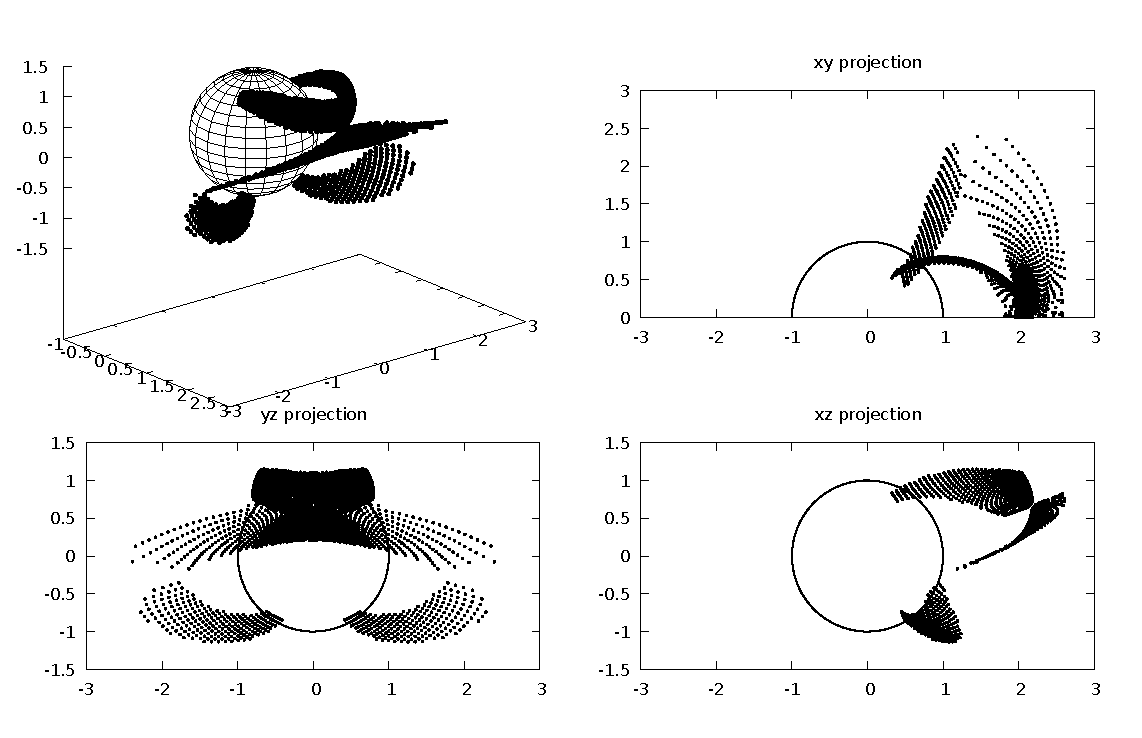
\includegraphics[width=1.0\textwidth]{surf.eps}
\caption{Рис.2. Резонансная поверхность магнитосферы для точки с координатами (2.2,0,0.7) (ось z вдоль оси магнитного поля). Слева-сверху: трехмерный вид (сфера - звезда). Справа-сверху: проекция на плоскость xy. Слева-снизу: проекция на плоскость yz. Справа-снизу: проекция на плоскость yz. Окружностью на плоских рисунках показана звезда.}
\end{figure}

\end{document}